% @Author: luis
% @Date:   2016-03-30 22:54:01
% @Last Modified by:   luis
% @Last Modified time: 2016-04-20 12:24:17

\documentclass[12pt]{article}
\usepackage{latexsym}
\usepackage{fancyhdr}
\usepackage{amssymb,amsmath,amsthm}
\usepackage[pdftex]{graphicx}
\usepackage{pdfpages}
\usepackage{hyperref}
\usepackage[margin=1in]{geometry}


% Create answer counter to keep track of seperate responses
\newcounter{AnswerCounter}
\newcounter{SubAnswerCounter}
\newcounter{SubSubAnswerCounter}
\setcounter{AnswerCounter}{1}
\setcounter{SubAnswerCounter}{1}
\setcounter{SubSubAnswerCounter}{1}

% Create answer environment which uses counter
\newenvironment{answer}[0]{
  \setcounter{SubAnswerCounter}{1}
  \bigskip
  \textbf{Solution \arabic{AnswerCounter}}
  \\
  \begin{small}
}{
  \end{small}
  \stepcounter{AnswerCounter}
}

\newenvironment{subanswer}[0]{
  \setcounter{SubSubAnswerCounter}{1}
  (\alph{SubAnswerCounter})
}{
 \bigskip
  \stepcounter{SubAnswerCounter}
}

\newenvironment{subsubanswer}[0]{
  \hspace{0.25in}[\roman{SubSubAnswerCounter}]
}{
 \bigskip
  \stepcounter{SubSubAnswerCounter}
}

% Allows easy use of vectors
\newcommand{\vect}[1]{\boldsymbol{#1}}
\newcommand{\deln}[3]{\frac{\partial^{#3} #1}{\partial #2^{#3}}}
\newcommand{\del}[2]{\frac{\partial#1}{\partial #2}}
\newcommand{\bra}[1]{\langle {#1} |}
\newcommand{\ket}[1]{| {#1} \rangle}
\newcommand{\dt}[2]{\langle {#1} | {#2} \rangle}
\newcommand{\braket}[3]{\langle {#1} | {#2} | {#3} \rangle}
\newcommand{\op}[1]{{#1}_{op}}
\newcommand{\opb}[1]{{\bf {#1}}_{op}}


% Custom Header information on each page
\pagestyle{fancy}
\lhead{HUID: 70871564}
\rhead{Luis Perez - \thepage}
\renewcommand{\headrulewidth}{0.1pt}
\renewcommand{\footrulewidth}{0.1pt}

\newcommand{\horrule}[1]{\rule{\linewidth}{#1}}   % Horizontal rule
\title{
    % \vspace{-1in}
    \usefont{OT1}{bch}{b}{n}
    \normalfont \normalsize \textsc{Harvard University} \\ [25pt]
    \horrule{0.5pt} \\[0.4cm]
    \huge Physics 143a: Quantum Mechanics I \\ [20pt]
    \normalfont \normalsize Problem Set 8
    \horrule{2pt} \\[0.5cm]
}
\author{
    \normalfont                 \normalsize
        Luis Antonio Perez\\[-3pt]    \normalsize
}
\date{\today}

\begin{document}
\maketitle
\pagebreak

\begin{answer}
We consider the hydrogenic radial wavefunction.

\begin{subanswer}
First, recall that the radial w.f. is given by:
$$
R_{nl}(r) \propto e^{-Zr/(na_B)}\left(\frac{2Zr}{na_B} \right)^l[L^{2l + 1}_{n-l-1}\left(\frac{2Zr}{na_B} \right)]
$$
and for $s$ states, (aka, $l = 0$), we have:
$$
R_{n0}(r) \propto e^{-Zr/(na_B)}[L^{1}_{n-1}\left(\frac{2Zr}{na_B} \right)] = -e^{-Zr/(na_B)}[\del{}{\rho}L_{n}\left(\frac{2Zr}{na_B} \right)]
$$
where $\rho = \frac{2Z r}{na_B}$ and $L_n^1$ is the associated Leguerre polynomial and $L_n$ the Leguerre polynomial. Then we consider the probability density for these $s$ states for some infinitesimal $dr$ which is proportional to:
$$
|r R_{n0}(r)|^2 dr = r^2 R_{n0}(r)^2 dr
$$
If we wish to find the maximum value of the above, we first note that we simply find the maximum or minimum value of the interior function:
$$
r R_{n0}(r)
$$
as the largest of these will become the maximum above. So taking the derivative of the interior, we have:
$$
R_{n0}(r) + r\del{}{r}R_{n0}(r) = 0
$$
which, plugging in what we know, yield:
\begin{align*}
-e^{-Zr/(na_B)}[\del{}{\rho}L_{n}\left(\frac{2Zr}{na_B} \right)] - e^{-Zr/(na_B)}[- r \frac{Z}{na_B}\del{}{\rho}L_{n}\left(\frac{2Zr}{na_B} \right) + \del{}{r}\del{}{\rho}L_{n}\left(\frac{2Zr}{na_B} \right)] &= 0 \\
\implies \del{}{\rho}L_{n}(\rho) + \rho \del{}{\rho}\del{}{\rho}L_n(\rho) - (\rho/2)\del{}{\rho}L_{n}(\rho) &=0
\end{align*}
and recalling the following:
$$
L_n(\rho) = e^{\rho}\deln{}{\rho}{n}(e^{-\rho}\rho^n)
$$
we note that:
\begin{align*}
\del{}{\rho}L_n(\rho) &=  \del{}{\rho}[e^{\rho}\deln{}{\rho}{n}(e^{-\rho}\rho^n)] \\
&= e^{\rho}\deln{}{\rho}{n}(e^{-\rho}\rho^n) + e^{\rho}\deln{}{\rho}{n}[\del{}{\rho}[(e^{-\rho}\rho^n)]] \\
&= e^{\rho}\deln{}{\rho}{n}(e^{-\rho}\rho^n) - e^{\rho}\deln{}{\rho}{n}(e^{-\rho}\rho^n) + ne^{\rho}\deln{}{\rho}{n}(e^{-\rho}\rho^{n-1})
\end{align*}
which is about as elementary as we will get. We can the use the above results to solve for the maximum.
If we solve the above, we will obtain the results. We do so for this first few levels of the hydrogen atom. Note that for $n = 1$, we have the following Leguerre polynomials:
\begin{align*}
L_1(x) &= -x - 1 \\
L_2(x) &= x^2 - 4x + 2
\end{align*}
so for $n = 1$ we have the following:
$$
-1 + (\rho/2) = 0 \implies \rho = 2 \implies \frac{2 Zr}{a_B} = 2 \implies r = \frac{a_B}{Z}
$$
and for $n = 2$ we have:
$$
(2\rho - 4) + 2\rho - (2\rho - 4)(\rho/2) = 0 \implies \rho^2 - 6\rho + 4 = 0 \implies r^2 - \frac{6a_B}{Z}r + \frac{4a_B^2}{Z^2} = 0
$$
which we can solve with the quadratic formula to obtain:
$$
r = \frac{6a_B \pm 2a_B\sqrt{5}}{2Z} = \frac{(3\pm\sqrt{5})a_B }{Z}
$$
we can continue as such, solving for higher degree polynomials. In this case, note that the maximum is the one that is given by:
$\frac{3 + \sqrt{5}}{Z}$.
\end{subanswer}

\begin{subanswer}
We look at the general form of the probability density for non-s states, which is given by:
$$
|r R_{nl}(r)|^2 dr = r^2 R_{nl}(r)^2 dr
$$
such that $l \neq 0$. Note that the value of the above at $r = 0$ can be calculated by first calculating the value of the interior. We have from Griffith that:
$$
r \to 0, R_{nl}(r) \to 0
$$
for $l \neq 0$. Therefore, it is immediate that the value of the probability density is precisely $0$. Mathematically, we show that for $l \neq 0$, $R_{nl}(r) \to 0$ as $r \to 0$. We can do this by considering the three terms that make up $R_{nl}(r)$ as $r \to 0$. We have:
\begin{align*}
e^{-Zr/(na_B)} \to 1 \\
\left(\frac{2Zr}{na_b} \right) \to 0 \\
L^{2l + 1}_{n-l-1}(x) = c
\end{align*}
The last line follows from the fact that the terms are polynomials, so they always converge to some constant value $c$. We therefore have that as $R_{nl}(r) \to 0$. The result fit with the intuition that for these levels, we don't have any probability density at the center. However, note that we did not use the fact that $l = 0$, so the above argument also holds for $s$-state wavefunctions.
\end{subanswer}

\begin{subanswer}
We define the circular state as having the maximum value of $l$ and $|m|$ for a given $n$. This means that $l = n -1$ and $m = \pm(n-1)$, where we'll take $m = n -1$ WLOG. Then we repeat the above analysis. Furthermore, note that the value of $m$ does not play a role since the spherical harmonics don't depend on $r$, and therefore they are simply constants and won't affect the minimum or the maximum. We wish to maximize/minimize the below:
$$
r R_{n(n-1)}(r) \propto r e^{-Zr/(na_B)}\left(\frac{2Zr}{na_B} \right)^{n-1}[L^{2n - 1}_{0}\left(\frac{2Zr}{na_B} \right)]
$$
Recalling the formula for $L_{q-p}^p(x) = (-1)^p \deln{}{x}{p} L_q(x)$, the formula $L_q(x) = e^x \deln{}{x}{q}e^{-x}x^q$, and plugging in $q = p$ (because $q-p = 0$), we have:
$$
r R_{n(n-1)}(r) \propto r e^{-Zr/(na_B)}\left(\frac{2Zr}{na_B} \right)^{n-1}
$$
where we've made used of the fact that
$$
\deln{}{x}{n}[e^x\deln{}{x}n (e^{-x}x^n)] = n!
$$
thereby dropping the term entirely.
So taking the derivative and setting equal to $0$, and simplifying notation a bit, we have:
\begin{align*}
e^{-\rho/2}\rho^{n-1} -  (\rho/2) e^{-\rho/2}\rho^{n-1} + (n-1) e^{-\rho/2}\rho^{n-1} &= 0 \\
\implies e^{-\rho/2}\rho^{n-1}[1 - (\rho/2) + (n-1)] &= 0 \\
\implies 1 - (\rho/2) + (n-1) = 0 \text{ or } \rho = 0
\end{align*}
The second equation gives us that $\rho = 0$ is a possible maximum/minimum. However, from the part above, we know that it is in fact a minimum, since the probability density is $0$ at this point. Therefore, we throw that out as a maximum. The second equation can be solved to give:
$$
\rho = 2n
$$
which we can solve to obtain:
$$
r = \frac{a_B}{Z}n^2
$$
\end{subanswer}

\begin{subanswer}
We define the probability distribution to simply be the probability density. We've already established the formula for it above, though we now repeat it:
$$
r R_{n(n-1)}(r) \propto  r e^{-Zr/(na_B)}\left(\frac{2Zr}{na_B} \right)^{n-1}
$$
and we point the reader to Figure \ref{fig:hydrogen}.
\begin{figure}[h!]
\centering
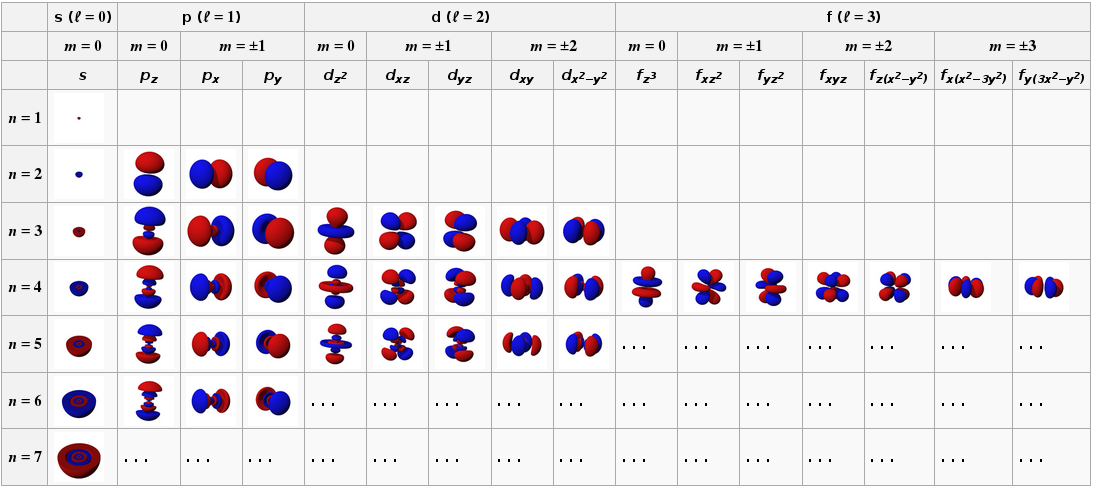
\includegraphics[scale=0.4]{orbitals.png}
\caption{Probability density for Hydrogen atom}
\label{fig:hydrogen}
\end{figure}
As can be seen, the formula is always has no probability density in the center. It is also symmetric above the multiple axes specified by $m$. The system has a lot of symmetry, as can be seen from both the forumla and the Figure. We now note some other properties. Not only is it the case that as $r \to 0$ the probability density $\to 0$ for these states, we also have that as $r \to \infty$ the first exponential terms decays much more quickly that the polynomial, and therefore we have that the probability density also approaches $0$. Another interesting property is the symmetric nature, which arises from two contributing factors: symmetry due to the rotations casued by $m$ (not that in our case, we're only focusing on the extreme values of $m$ which are degenerate (equivalent states, even under rotation). The second element of symmetry arises from the squaring function. Recall that we've defined th probability density as:
$$
|rR_{nl}(r)|^2 dr
$$
which gives us, in the image, the red and blue ovals. There are meant to represent the fact that some of the orbitals interact destructively.
\end{subanswer}
\end{answer}

\begin{answer}
We now consider the state that is made of the direct product of a state with $j_1 = 1$ and $j_2 = \frac{3}{2}$.
$$
\sqrt{\frac{3}{5}}\ket{1,-1}\ket{\frac{3}{2},-\frac{1}{2}} + \sqrt{\frac{2}{5}}\ket{1,0}\ket{\frac{3}{2},-\frac{3}{2}}
$$

\begin{subanswer}
We now show that the above is an eigenstate for the total angular momentum operator $J^2$ where we define $J \equiv J_1 + J_2$ where $J_1,J_2$ are the respective operators of the states $j_1$ and $j_2$.
\begin{align*}
&J^2 \left[ \sqrt{\frac{3}{5}}\ket{1,-1}\ket{\frac{3}{2},-\frac{1}{2}} + \sqrt{\frac{2}5}\ket{1,0}\ket{\frac{3}{2},-\frac{3}{2}} \right]\\
&= J^2\sqrt{\frac{3}{5}}\ket{1,-1}\ket{\frac{3}{2},-\frac{1}{2}} + J^2\sqrt{\frac{2}{5}}\ket{1,0}\ket{\frac{3}{2},-\frac{3}{2}} \\
&= (J_1 + J_2)^2\sqrt{\frac{3}{5}}\ket{1,-1}\ket{\frac{3}{2},-\frac{1}{2}} + (J_1 + J_2)^2\sqrt{\frac{2}{5}}\ket{1,0}\ket{\frac{3}{2},-\frac{3}{2}} \\
&= (J_1^2 + J_2^2 + 2J_1 \cdot J_2) \sqrt{\frac{3}{5}}\ket{1,-1}\ket{\frac{3}{2},-\frac{1}{2}} + (J_1^2 + J_2^2 + 2J_1 \cdot J_2)\sqrt{\frac{2}{5}}\ket{1,0}\ket{\frac{3}{2},-\frac{3}{2}} \\
&= (2\hbar^2 + \left(\frac{3}{2}\right)\left(\frac{5}{2}\right)\hbar^2)\sqrt{\frac{3}{5}}\ket{1,-1}\ket{\frac{3}{2},-\frac{1}{2}} + (2 \hbar^2 + \left(\frac{3}{2}\right)\left(\frac{5}{2}\right)\hbar^2)\sqrt{\frac{2}{5}}\ket{1,0}\ket{\frac{3}{2},-\frac{3}{2}} \\
&+ (2J_1\cdot J_2)\left[\sqrt{\frac{3}{5}}\ket{1,-1}\ket{\frac{3}{2},-\frac{1}{2}} + \sqrt{\frac{2}{5}}\ket{1,0}\ket{\frac{3}{2},-\frac{3}{2}}\right]
\end{align*}
NOTE: Continued on attached paper. Did not have time to finish LaTeXing. Apologies!

Best wishes,

Luis
\end{subanswer}

\begin{subanswer}
On sheet.
\end{subanswer}

\begin{subanswer}
On sheet.
\end{subanswer}
\end{answer}

\begin{answer}
On separate sheet.

\end{answer}

\begin{answer}
For the verifications with Mathematica, see the attached notebook.

\begin{subanswer}
We have the following state, according to the tables:
$$
\ket{(1, \frac{1}{2}),\frac{1}{2},-\frac{1}{2} } = \sqrt{\frac{1}{3}}\ket{1,0}\ket{\frac{1}{2},-\frac{1}{2}} - \sqrt{\frac{2}{3}}\ket{1,-1}\ket{\frac{1}{2},\frac{1}{2}}
$$
which we verified with Mathematica.
\end{subanswer}

\begin{subanswer}
We have the following state, according to the tables:
$$
\ket{(1, \frac{1}{2}),\frac{3}{2},\frac{1}{2} } = \sqrt{\frac{1}{3}}\ket{1,1}\ket{\frac{1}{2},-\frac{1}{2}} + \sqrt{\frac{2}{3}}\ket{1,0}\ket{\frac{1}{2},\frac{1}{2}}
$$
which we verified with Mathematica.
\end{subanswer}

\begin{subanswer}
We have the following state, according to Mathematica (since the table doesn't go this high!):
$$
\ket{(\frac{7}{2}, \frac{3}{2}),4,-2 } = \sqrt{\frac{3}{40}}\ket{\frac{7}{2},-\frac{7}{2}} \ket{\frac{3}{2},\frac{3}{2}} + \sqrt{\frac{121}{280}}\ket{\frac{7}{2},-\frac{5}{2}}\ket{\frac{3}{2},\frac{1}{2}} + \sqrt{\frac{3}{280}} \ket{\frac{7}{2},-\frac{3}{2}}\ket{\frac{3}{2},\frac{1}{2}} + \sqrt{\frac{27}{56}}\ket{\frac{7}{2},-\frac{1}{2}}\ket{\frac{3}{2},-\frac{3}{2}}
$$
which we can see, at the very least, the squared coefficients sum to 1!
\end{subanswer}


\end{answer}

\end{document}